\documentclass[10pt]{article}
\renewcommand{\baselinestretch}{1.8}

\usepackage[b4paper,left=0.8in,right=0.8in,top=0.8in,bottom=0.8in]{geometry}
\usepackage{tikz-qtree}
\usepackage{algorithm}
\usepackage{algpseudocode}
\makeatletter
\renewcommand{\ALG@beginalgorithmic}{\footnotesize}
\makeatother
\usepackage{graphicx}
\usepackage{subcaption}
\usepackage{showkeys}
\usepackage{amsmath}


\usepackage{multicol}
\setlength\columnsep{24pt}

\algnewcommand\algorithmicforeach{\bf{for each}}
\algdef{S}[FOR]{ForEach}[1]{\algorithmicforeach\ #1\ \algorithmicdo}

\algdef{S}[FUNCTION]{Function}
   [3]{{\tt{\sl{#1}}} \textproc{\tt{#2}}\ifthenelse{\equal{#3}{}}{}{\tt{(#3)}}}
  
\algdef{E}[FUNCTION]{EndFunction}
   [1]{\algorithmicend\ \tt{\textproc{#1}}}

\algrenewcommand\Call[2]{\tt{\textproc{#1}\ifthenelse{\equal{#2}{}}{}{(#2)}}}
   
\newcommand\keywordfont{\sffamily\bfseries}
\algrenewcommand\algorithmicend{{\keywordfont end}}
\algrenewcommand\algorithmicfor{{\keywordfont for}}
\algrenewcommand\algorithmicforeach{{\keywordfont for each}}
\algrenewcommand\algorithmicdo{{\keywordfont do}}
\algrenewcommand\algorithmicuntil{{\keywordfont until}}
\algrenewcommand\algorithmicfunction{{\keywordfont function}}
\algrenewcommand\algorithmicif{{\keywordfont if}}
\algrenewcommand\algorithmicthen{{\keywordfont then}}
\algrenewcommand\algorithmicelse{{\keywordfont else}}
\algrenewcommand\algorithmicreturn{{\keywordfont return}}

\renewcommand\thealgorithm{}
\newcommand{\setalglineno}[1]{%
  \setcounter{ALC@line}{\numexpr#1-1}}

\newcommand{\sub}[1]{\textsubscript{#1}}
\renewcommand{\tt}[1]{\texttt{#1}}
\renewcommand{\sl}[1]{\textsl{#1}}
\renewcommand{\it}[1]{\textit{#1}}
\renewcommand{\sc}[1]{\textsc{#1}}
\renewcommand{\bf}[1]{\textbf{#1}}
\newcommand{\nf}[1]{{\normalfont{\texttt{#1}}}}
\newcommand{\cmt}[1]{\Comment{#1}}
\newcommand{\head}{head}
\newcommand{\size}{size }

\usepackage{amsmath,amssymb,amsthm}
\newtheorem{theorem}{Theorem}
\newtheorem{lemma}[theorem]{Lemma}
\newtheorem{corollary}[theorem]{Corollary}
\newtheorem{observation}[theorem]{Observation}
\theoremstyle{definition}
\newtheorem{definition}[theorem]{Definition}
\newtheorem{invariant}[theorem]{Invariant}

\begin{document}

\section{Pseudocode}

\begin{algorithm}
\caption{Tree Fields Description}
\begin{algorithmic}[1]
\setcounter{ALG@line}{100}
\begin{multicols}{2}

%\Statex \bf{Structure}

\Statex $\diamondsuit$ \tt{\sl{Shared}}
\begin{itemize}
\item \textsf{A binary tree of \tt{Node}s with one \tt{leaf} for each process. \tt{root} is the root \nf{node}.}
%such that \tt{root} is the root and the left child and the right child and the parent of \tt{Tree[i]} are \tt{Tree[2i+1]}, \tt{Tree[2i+2]} and \tt{Tree[i/2]}.
\end{itemize}

\Statex

\Statex $\diamondsuit$ \tt{\sl{Local}}
\begin{itemize}
\item \tt{\sl{Node} leaf:} \sf{ process's leaf in the tree.}
\end{itemize}

\Statex
\Statex $\diamondsuit$ \tt{\sl{Structures}}

\Statex $\blacktriangleright$ \tt{\sl{Node}}
\begin{itemize}
\item \tt{\sl{*Node} left, right, parent} \textsf{: initialized  when creating the tree.}
\item \tt{\sl{BlockList}}
\item \tt{\sl{int} \head= 1}\textsf{: \#\tt{block}s in \tt{blocks}. \tt{blocks[0]} is a block with all integer fields equal to zero.}
\item \tt{\sl{int} num\sub{propagated}= 0}\textsf{} \textsf{: \# groups of blocks that have been propagated from the node to its parent. Since it is incremented after propagating, it may be behind by 1.}
\end{itemize}

%\Statex $\blacktriangleright$ \tt{\sl{Root} extends \sl{Node}}
%\begin{itemize}
%  
%\item \tt{\sl{PBRT} blocks}
%
%  \textsf{\tt{BlockList} is implemented with a persistent red-black tree.}
%  
%\end{itemize}

%\Statex $\blacktriangleright$ \tt{\sl{NonRootNode} extends \sl{Node}}
%\begin{itemize}
    
%\end{itemize}

%\Statex $\blacktriangleright$ \tt{\sl{Leaf} extends \sl{Node}}
%\begin{itemize}
%  
%  \item \tt{\sl{int} \tt{last\sub{done}}}
%
%  \textsf{Stores the index of the block in the root such that the process that owns this leaf has most recently finished the. A block is finished if all of its operations are finished. \tt{enqueue(e)} is finished if \tt{e} is returned by some \tt{dequeue()} and \tt{dequeue()} is finished when it computes its response. \it{put the definitions before the pseudocode}}
%  
%\end{itemize}

\Statex $\blacktriangleright$ \tt{\sl{Block}} 
%\cmt{If \tt{b} is \tt{blocks[i](i!=0)} then \tt{b[-1] is blocks[i-1].}}

\begin{itemize}
%  \item \tt{\sl{int} num\sub{enq}, num\sub{deq}}
%  \textsf{: \# enqueue, dequeue operations in the block}
%  \item \tt{\sl{int} num, sum}
%  \textsf{: total \# operations in block, prefix sum of \tt{num}}

  \item \tt{\sl{int} group}
  \textsf{: the value read from \tt{num\sub{propagated}} when appending this block to the node.}
\end{itemize}

\pagebreak


\Statex $\blacktriangleright$ \tt{\sl{LeafBlock} extends \sl{Block}}
\begin{itemize}
  \item \tt{\sl{Object} element}
  \textsf{: Each block in a leaf represents a single operation. If the operation is \tt{enqueue(x)} then \tt{element=x}, otherwise \tt{element=null}.}
  
    \item \tt{\sl{int} sum\sub{enq}, sum\sub{deq}}
  \textsf{: \# enqueue, dequeue operations in the prefix for the block}
  
\end{itemize}



\Statex $\blacktriangleright$ \tt{\sl{InternalBlock} extends \sl{Block}}
\begin{itemize}
    \item \tt{\sl{int} end\sub{left}, end\sub{right}}
  \textsf{:~~indices of the last subblock of the block in the left and right child}
  \item \tt{\sl{int} sum\sub{enq-left}}
  \textsf{: \# enqueue operations in the prefix for \tt{left.blocks[end\sub{left}]}}
  \item \tt{\sl{int} sum\sub{deq-left}}
  \textsf{: \# dequeue operations in the prefix for \tt{left.blocks[end\sub{left}]}}
  \item \tt{\sl{int} sum\sub{enq-right}}
  \textsf{: \# enqueue operations in the prefix for \tt{right.blocks[end\sub{right}]}}
  \item \tt{\sl{int} sum\sub{deq-right}}
  \textsf{: \# dequeue operations in the prefix for \tt{right.blocks[end\sub{right}]}}
\end{itemize}


\Statex $\blacktriangleright$ \tt{\sl{RootBlock} extends \sl{InternalBlock}}
\begin{itemize}
  \item \tt{\sl{int} \size}
  \textsf{: size of the queue after performing all operations in the prefix for this block}
%  \item \tt{\sl{int} sum\sub{non-null deq}}
%  \textsf{: count of non-null dequeus up to this block}
%  \item \tt{\sl{counter} num\sub{finished}}
%  \textsf{: number of finished operations in the block}
%    \item \tt{\sl{int} order}
%  \textsf{: the index of the block in the \tt{BlockList} containing the block.}
\end{itemize}

%\Statex $\blacktriangleright$ \tt{Conventions}
%\begin{itemize}
%  \item \tt{i} : index of ith operation in the tree
%  \item \tt{j} : index of jth operation in a node
%  \item \tt{b\sub{n}} : index of the block containing the operation n based on the scope
%  \item Also we are not going to refer to blocks directly, only with their indices. Except while constructing a new block.
%\end{itemize}


\end{multicols}
\end{algorithmic}
\end{algorithm}

%##########################################

\begin{footnotesize}
  
%\it{Variable naming:}
%\begin{itemize}
%  \item \tt{b\sub{op}}: index of the block containing operation \tt{op}
%  \item \tt{r\sub{op}}: rank of operation \tt{op} i.e. the ordering among the operations of its type according to linearization ordering
%\end{itemize}

\it{Abbreviations:}
\begin{itemize}
 \item \tt{blocks[b].sum\sub{x}=blocks[b].sum\sub{x-left}+blocks[b].sum\sub{x-right}}  \tt{ (for b$\geq$0 and x $\in$ \{enq, deq\}})
 \item \tt{blocks[b].sum=blocks[b].sum\sub{enq}+blocks[b].sum\sub{deq}}  \tt{ (for b$\geq$0})
  \item \tt{blocks[b].num\sub{x}=blocks[b].sum\sub{x}-blocks[b-1].sum\sub{x}} \\ \tt{(for b>0 and x $\in$ \{$\emptyset$, enq, deq, enq-left, enq-right, deq-left, deq-right\})}
\end{itemize}
\end{footnotesize}

\pagebreak

%##########################################


\begin{algorithm}
\caption{\tt{\sl{Queue}}}
\begin{algorithmic}[1]
\setcounter{ALG@line}{200}
\begin{multicols}{2}

\Function{void}{Enqueue}{\sl{Object} e} \cmt{Creates a \tt{block} with element \tt{e} and adds it to the tree.}
\State \tt{block newBlock= \Call{new}{\sl{LeafBlock}}}
\State \tt{newBlock.element= e}
%\State \tt{b.num\sub{enq}=1}
\State \tt{newBlock.sum\sub{enq}= leaf.blocks[leaf.\head].sum\sub{enq}+1}
\State \tt{newBlock.sum\sub{deq}= leaf.blocks[leaf.\head].sum\sub{deq}}
\State \tt{leaf.}\Call{Append}{newBlock}
\EndFunction{Enqueue}

\Statex

\Function{Object}{Dequeue()}{} \cmt{Creates a block with null value element, appends it to the tree, computes its order among operations, and returns its response.}
\State \tt{block newBlock= \Call{new}{\sl{LeafBlock}}} 
\State \tt{newBlock.element= null}
\State \tt{newBlock.sum\sub{enq}= leaf.blocks[leaf.\head].sum\sub{enq}}
\State \tt{newBlock.sum\sub{deq}= leaf.blocks[leaf.\head].sum\sub{deq}+1}
\State \tt{leaf.}\Call{Append}{newBlock}
\State \tt{<b, i>=} \Call{IndexDeq}{leaf.\head, 1}
\State \tt{output=} \Call{FindResponse}{b, i} 
\label{deqRest}
%\If{\tt{i\sub{enq}==-1}}
%\State \tt{output= null}
%\Else
%\State \tt{output= \Call{GetEnq}{b\sub{enq}, i\sub{enq}}}
%\EndIf
\State \Return{\tt{output}}
\EndFunction{Dequeue}

\pagebreak

\Function{<int, int>}{FindResponse}{\sl{int} b, \sl{int} i}\Statex\cmt{Returns the the response to the $D_{root,b,i}$.}
\If{\tt{ root.blocks[b-1].\size}\tt{ + root.blocks[b].num\sub{enq} - i $<$ 0}} \State \Return \tt{null} \label{checkEmpty}\cmt{Check if the queue is empty.}
\Else
\State \tt{e= i - root.blocks[b-1].size + root.blocks[b-1].sum\sub{enq}} \label{computeE}
\Statex\cmt{$E_{root,e}$ is the response.}
\State \Return \tt{root.GetENQ(root.\Call{DSearch}{e, b})}\label{findAnswer}
\EndIf
\EndFunction{FindResponse}

\end{multicols}
\end{algorithmic}
\end{algorithm}
%##########################################


\begin{algorithm}
\caption{\tt{\sl{Node}}}
\begin{algorithmic}[1]
\setcounter{ALG@line}{300}
\begin{multicols}{2}

\Function{void}{Propagate()}{}
\If{\bf{not} \Call{Refresh()}{}} \label{firstRefresh}
\State \Call{Refresh()}{} \label{secondRefresh}
\EndIf
\If{\tt{this} \bf{is not} \tt{root}}
\State \tt{parent.}\Call{Propagate()}{}
\EndIf
\EndFunction{Propagate}

\Statex

\Function{boolean}{Refresh()}{}
\State \tt{h= \head} \label{readHead}
%\If{\tt{n.blocks[h]!=null?}} \tt{h+=1}\EndIf
\State \tt{<new, np\sub{left}, np\sub{right}>= \Call{CreateBlock}{h}} \label{invokeCreateBlock} \cmt{\tt{np\sub{left}, np\sub{right}} are the values read from the children's \tt{num\sub{propagated}} field.}
\If{\tt{new.num==0}} \Return{\tt{true}} \label{addOP} \cmt{The block contains nothing.}
\ElsIf{\tt{blocks.tryAppend(new, h)}} \label{cas}
\ForEach{\tt{dir} {\keywordfont{in}} \tt{\{left, right\}}} \label{okcas}
\State \tt{\Call{CAS}{dir.super[np\sub{dir}], null, h}} \cmt{Write would work too.} \label{setSuper}
\State \tt{\Call{CAS}{dir.num\sub{propagated}, np\sub{dir}, np\sub{dir}+1}} \label{incNP}
\EndFor
\State \tt{\Call{CAS}{\head, h, h+1}} \label{incrementHead1}
\State \Return{\tt{true}}
\Else
\State \tt{\Call{CAS}{\head, h, h+1}} \cmt{Even if another process wins, help to increase the \tt{\head}. The winner might have fallen sleep before increasing \tt{\head}.} \label{incrementHead2}
\State \Return{ \tt{false}}
\EndIf
\EndFunction{Refresh}

\Statex

\Statex $\leadsto$ \textsf{Precondition: \tt{blocks[start..end]} contains a block with field \tt{f} $\geq$ \tt{i}}
\Function{int}{BSearch}{\sl{field} f, \sl{int} i, \sl{int} start, \sl{int} end}

\Statex \cmt{\textmd{Does binary search for~the value \tt{i} of the given prefix sum \tt{field}. Returns the index of the leftmost block in \tt{blocks[start..end]} whose \sl{field} \tt{f} is $\geq$ \tt{i}}.}
%\State \Return \tt{result block's index}
\EndFunction{BSearch}



\pagebreak

\Function{<Block, int, int>}{CreateBlock}{\sl{int} i} 
\cmt{Creates a block to be inserted as $i$th \tt{block} in \tt{blocks}. Returns the created block as well as values read from each child's \tt{num\sub{propagated}} field. These values are used for incrementing the children's \tt{num\sub{propagated}} field if the block was appended to \tt{blocks} successfully.}
\State \tt{block newBlock= \Call{new}{\sl{block}}}
\State \tt{newBlock.group= num\sub{propagated}}\label{setGroup}
\ForEach{\tt{dir} {\keywordfont{in}} \tt{\{left, right\}}}
\State \tt{index\sub{last}= dir.\head} \label{lastLine}
\State \tt{index\sub{prev}= blocks[i-1].end\sub{dir}} \label{prevLine}
\State \tt{newBlock.end\sub{dir}= index\sub{last}} \label{endDefLine}
\State \tt{block\sub{last}= dir.blocks[index\sub{last}]}
\State \tt{block\sub{prev}= dir.blocks[index\sub{prev}]}
\State \cmt{\tt{newBlock} includes \tt{dir.blocks[index\sub{prev}+1..index\sub{last}]}.}
\State \tt{np\sub{dir}= dir.num\sub{propagated}} \label{setNP}
\State \tt{newBlock.sum\sub{enq-dir}= blocks[i-1].sum\sub{enq-dir} + block\sub{last}.sum\sub{enq} - block\sub{prev}.sum\sub{enq}}
\State \tt{newBlock.sum\sub{deq-dir}= blocks[i-1].sum\sub{deq-dir} + block\sub{last}.sum\sub{deq} - block\sub{prev}.sum\sub{deq}}
\EndFor
%\State \tt{b.num\sub{enq}= b.num\sub{enq-left} + b.num\sub{enq-right}}
%\State \tt{b.num\sub{deq}= b.num\sub{deq-left} + b.num\sub{deq-right}}
%\State \tt{b.num= b.num\sub{enq} + b.num\sub{deq}}
%\State \tt{b.sum= n.blocks[i-1].sum + b.num}

\If{\tt{this} \bf{is} \tt{root}}
\State \tt{newBlock.\size= max(root.blocks[i-1].\size { }+ newBlock.num\sub{enq} - newBlock.num\sub{deq}, 0)}\label{computeLength}
%\State \tt{b.sum\sub{non-null deq}= root.blocks[i-1].sum\sub{non-null deq} + max( b.num\sub{deq} - root.blocks[i-1].length - b.num\sub{enq}, 0)}
\EndIf

\State \Return \tt{<b, np\sub{left}, np\sub{right}>}
\EndFunction{CreateBlock}

\end{multicols}
\end{algorithmic}
\end{algorithm}
\begin{algorithm}
\caption{Root}
\begin{algorithmic}[1]
\setcounter{ALG@line}{800}
\Statex
\Statex $\leadsto$ \textsf{Precondition: \tt{root.blocks[end].sum\sub{enq} $\geq$ \tt{e}}}
\Function{<int, int>}{DSearch}{\sl{int} e, \sl{int} end}
\cmt{Returns \tt{<b,i>} if $E_{root,e}=E_{root,b,i}$.}
\State \tt{start= end-1}
\While{\tt{root.blocks[start].sum\sub{enq}}$\geq$\tt{e}}
\State \tt{start= max(start-(end-start), 0)} \label{doubling}
\EndWhile
\State \tt{b= root.BSearch(sum\sub{enq}, e, start, end)}
\State \tt{i= e- root.blocks[b-1].sum\sub{enq}} \label{DSearchComputei}
\State\Return \tt{<b,i>}
\EndFunction{DSearch}
\end{algorithmic}
\end{algorithm}

%##########################################

\begin{algorithm}
\caption{Node}
\begin{algorithmic}[1]
\setcounter{ALG@line}{400}

\Statex $\leadsto$ \textsf{Precondition:~\tt{blocks[b].num\sub{enq}$\geq$i}}
\Function{element}{GetEnq}{\sl{int} b, \sl{int} i} \cmt{Returns the element of $E_{this,b,i}$.}
\If{\tt{this} \bf{is} \tt{leaf}}
\State\Return \tt{blocks[b].element} \label{getBaseCase}
\ElsIf{\tt{i $\leq$ blocks[b].num\sub{enq-left}}} \label{leftOrRight} \cmt{$E_{this,b,i}$ is in the left child of this node.}
\State \tt{subBlock= left.\Call{BSearch}{sum\sub{enq}, i+blocks[b-1].sum\sub{enq-left}, blocks[b-1].end\sub{left}+1, blocks[b].end\sub{left}}} \label{leftChildGet}
\State \Return\tt{left.}\Call{GetEnq}{subBlock, i} 
\Else
\State \tt{i= i-blocks[b].num\sub{enq-left}}
\State\tt{subBlock= right.\Call{BSearch}{sum\sub{enq}, i+right.blocks[b-1].sum\sub{enq-right}, blocks[b-1].end\sub{right}+1, blocks[b].end\sub{right}}} \label{rightChildGet}
\State \Return\tt{right.}\Call{GetEnq}{subBlock, i} 
\EndIf
\EndFunction{GetEnq}

\Statex
\Statex $\leadsto$ \textsf{Precondition: \tt{b}th block of the node has propagated up to the root and \tt{blocks[b].num\sub{enq}$\geq$i}.}
\Function{<int, int>}{IndexDeq}{\sl{int} b, \sl{int} i} \cmt{Returns \tt{<x, y>} if $D_{this,b,i}=D_{root,x,y}$.}
\If{\tt{this} \bf{is} \tt{root}}
\State\Return \tt{<b, i>} \label{indexBaseCase}
\Else
\State \tt{dir= (parent.left==n)? left: right} \cmt{check if this node is a left or a right child}
\State \tt{superBlock= parent.\Call{BSearch}{sum\sub{deq-dir}, i+blocks[b-1].sum\sub{deq}, super[blocks[b].group]-p, super[blocks[b].group]+p}} \label{computeSuper}
\Statex\cmt{superblock's group has at most $p$ difference with the value stored in \tt{super[]}.}
\If{\tt{dir {\keywordfont is} right}}
%\State \tt{i+= parent.blocks[superBlock-1].sum\sub{deq-right}}
\State \tt{i+= blocks[superBlock].num\sub{deq-left}} \cmt{consider the dequeues from the right child} \label{considerRight}
\EndIf
\State \Return\tt{this.parent.}\Call{IndexDeq}{superBlock, i}
\EndIf
\EndFunction{IndexDeq}

\end{algorithmic}
\end{algorithm}


%##########################################

%\begin{algorithm}
%\caption{Root}
%\begin{algorithmic}[1]
%\setcounter{ALG@line}{500}
%
%\Function{Block}{FindMostRecentDone}{}
%\For{\tt{leaf l} \bf{in leaves}}
%\State\tt{max= Max(l.maxOld, max)}
%\EndFor
%\State\Return\tt{max} \cmt{This snapshot suffies.}
%\EndFunction{FindMostRecentDone}
%
%\end{algorithmic}
%\end{algorithm}
%##########################################

\begin{algorithm}
\caption{Leaf}
\begin{algorithmic}[1]
\setcounter{ALG@line}{600}

\Function{void}{Append}{\sl{block} blk} \cmt{Append is only called by the owner of the leaf.}
\State \tt{\head+=1} \label{appendEnd} 
\State \tt{blk.group= \head} \label{appendStart} 
\State \tt{blocks[\head]= blk} 
\State \tt{parent.}\Call{Propagate()}{} 
\EndFunction{Append}

%\Statex
%
%\Function{void}{Help}{}\cmt{Helps pending operations}
%
%\State{\tt{last= l.\head-1}}
%\cmt{\tt{l.blocks[last]} can not be \tt{null} because \head increases after appending, see lines \ref{appendStart}-\ref{appendEnd}.}
%\If{\tt{l.blocks[last].element==null}} \cmt{operation is dequeue}
%\State \tt{l.blocks[last].response= l.}\Call{HelpDequeue()}{}
%\EndIf
%
%\EndFunction{Help}

\end{algorithmic}
\end{algorithm}

\begin{algorithm}
\caption{BlockList}
\begin{algorithmic}[1]
\setcounter{ALG@line}{700}

\Statex \cmt{\textsf{: Supports two operations \tt{blocks.tryAppend(Block b), blocks[i]}. Initially  empty, when \tt{blocks.tryAppend(b, n)} returns true \tt{b} is appended to \tt{blocks[n]} and \tt{blocks[i]} returns $i$th block in the \tt{blocks}. If some instance of \tt{blocks.tryAppend(b, n)} returns \tt{false} there is a concurrent instance of \tt{blocks.tryAppend(b$^\prime$, n)} which has returned \tt{true}.\tt{blocks[0]} contains an empty block with all fields equal to 0 and \tt{end\sub{left}, end\sub{right}} pointers to the first block of the corresponding children.}}

%\Statex
%\Statex $\diamondsuit$ \tt{\sl{root implementation}}
%%  \Statex \sf{A persistant red-black tree supporting \tt{append(b, key),get(key=i),split(j)}}.
%%  \tt{append(b, key) returns \tt{true} in case successful. Since \tt{order, sum\sub{enq}}are both strictly increasing we can use one of them for another.}
%%\Statex \tt{root: }\sf{pointer to the root of the PBRT}
%\Function{boolean}{TryAppend}{\sl{block} blk, \sl{int} n} \cmt{\textsf{adds block b to the \tt{root.blocks[n]}}}
%\If{\tt{root.size\%$p^2$==0}} \cmt{Help every often $p^2$ operations appended to the root.}
%\For{\tt{leaf l} \bf{in} \tt{tree leaves}}
%\State \tt{l.Help()}
%\EndFor
%\EndIf
%\State \tt{blk.num\sub{finished}= 0}
%%\State \tt{*oldRoot= \&root.blocks.root}
%%\State \tt{*newRoot= root.blocks.Append(blk).root}
%%\State \Return \tt{CAS(root, oldRoot, newRoot)}
%\State \Return{\tt{CAS(blocks[n], null, blk)}}
%\EndFunction{TryAppend}

\Statex
%\Statex $\diamondsuit$ \tt{\sl{Array implementation}}
\Statex \tt{\sl{block[]} blocks: }\sf{array of blocks}
\Statex \tt{\sl{int[]} super}\textsf{: \tt{super[i]} stores an approximate index of the superblock of the blocks in \tt{blocks} whose \tt{group} field have value \tt{i}.}
\Statex
\Function{boolean}{TryAppend}{\sl{block} blk, \sl{int} n} 
\State \Return{\tt{CAS(blocks[n], null, blk)}}
\EndFunction{TryAppend}


\end{algorithmic}
\end{algorithm}


%##########################################


%\begin{algorithm}
%\caption{Yet to decide how to handle.}
%\begin{algorithmic}[1]
%\setcounter{ALG@line}{800}
%
%%\Function{void}{CollectGarbage}{}\cmt{Collects the root blocks that are done.}
%%\State \tt{s=FindMostRecentDone(Root.Blocks.root)}  \cmt{Lemma: If block b is done after helping then all blocks before b are done as well.}
%%\State \tt{t1,t2= RBT.split(order, s)}
%%\State \tt{RBTRoot.CAS(t2.root)}
%%\EndFunction{CollectGarbage}
%
%\Function{response}{FallBack}{op i} \cmt{\it{how to use as exception handling? by adding try catch in all the methods reading the root?}}
%
%\If{root.blocks.get(num\sub{enq}), i is null} \cmt{this enqueue was already finished}
%
%\State \Return \tt{this.leaf.response(block.order)}
%\EndIf
%
%\EndFunction{FallBack}
%
%\end{algorithmic}
%\end{algorithm}

%%%%%%%%%%%%%%%%%%%%%%%%%%%%%%%%%%%%%%%%%%%%%
                     %
                     %
                     %
                     %
                     %
                     %
                     %
%%%%%%%%%%%%%%%%%%%%%%%%%%%%%%%%%%%%%%%%%%%%%

\clearpage

\section{Proof of Linearizability}

\framebox[1.1\width]{TEST} Fix the logical order of definitions (cyclic refrences).

%\framebox[1.1\width]{Questions} When I write the lemmas since every claim in my mind is correct maybe I miss some fact that need proof or maybe I refer to some lemmas that are generally correct but not needed for the linearizability proof. Is lemma 7 necessary? Is lemma 13 induced trivially from lemma 8?

\framebox[1.1\width]{TEST} Is it better to show \nf{ops(EST\sub{n, t})} with \nf{EST\sub{n, t}}?

%\framebox[1.1\width]{TEST} How to merge notions of blocks and operations? block b $\sqsubseteq$ block c means b is subblock of c. block b $\in$ set B means b is in B. Merge these two to have shorter formulaes.

\framebox[1.1\width]{Question} A good notation for \it{the index of the \nf{b}}?

\framebox[1.1\width]{Question} How to remove the notion of time? To say pre(n,i) contains n.blocks[0..i] instead of EST(n,t) which head=i at time t. Is it good? Furthermore, can we remove the notion of established blocks?

\begin{definition}[Block]
A block is an object storing some statistics, as described in Algorithm Queue. It implicitly represents a set of operations. If \nf{n.blocks[i]==b}  we call \nf{i} the \emph{index} of block \nf{b}. Block \nf{b} is before block \nf{b$^\prime$} in node \nf{n} if and only if the index of the \nf{b} is smaller than the index of the \nf{b$^\prime$}'s. For a \tt{block} in a \tt{BlockList} we define \it{the prefix for the block} to be the blocks in the \tt{BlockList} up to and including the \tt{block}.
\end{definition}

\begin{invariant}[headPosition] \label{lem::headPosition} If the value of \nf{n.head} is \nf{h} then, \nf{n.blocks[i]=null} for \nf{i>h} and \nf{n.blocks[i]$\neq$null} for \nf{i<h}.
\end{invariant}
\begin{proof}
The invariant is true initially since 1 is assigned to \nf{n.head} and \nf{n.blocks[x]} is null for every \nf{x}. The truth of the invariant may be affected by writing into \nf{n.blocks} or incrementing \nf{n.head}.

Some value is written into \nf{n.blocks[head]} only in Line 313. It is obvious that writing into \nf{n.blocks[head]} presereves the invariant. The value of \nf{n.head} is modified only in lines \ref{incrementHead1}], \ref{incrementHead2}. Depending on wether the \nf{TryAppend()}in Line\ref{cas} succeeded or not we show that the claim holds after the increment lines of \nf{n.head} in either case. If \nf{head} is incremented to $h$ it is sufficient to show \nf{n.blocks[h]}$\neq$\nf{null} to prove the invariant still holds. In the first case the process applied a successful \nf{TryAppend(new,h)} in line \ref{okcas}, which means \nf{n.blocks[h]} is not null anymore. Note that wether\ref{incrementHead1} returns true or false after Line \nf{n.head} we know has been incremented from Line \ref{readHead}. The failure case is also the same since it means some value is written into \nf{n.blocks[head]} by some process.
%At the end of every \nf{n.Refresh()} with a block  with \head greater than 0 returned by \nf{CreateBlock()} \nf{n.head} is incremented (Lines \ref{incrementHead1}, \ref{incrementHead2}). If a process went to sleep before incrementing the \nf{established} (line \ref{incrementHead1}), nothing can be appended to \nf{n.blocks} until another process increments \nf{n.establsihed} (Line \ref{incrementHead2}).
\end{proof}
\it{Explain More}

\begin{lemma}[headProgress] \label{lem::headProgress}
\nf{n.head} is non-decreasing over time and \nf{n.blocks[i].end\sub{left}} $\geq$ \nf{n.blocks[i-1].end\sub{left}} and \nf{n.blocks[i].end\sub{right}} $\geq$ \nf{n.blocks[i-1].end\sub{right}}.
\end{lemma}
\begin{proof}
The first claim follows trivially from the pseudocode since \nf{n.head} is only incremented in the pseudocode in the lines \ref{incrementHead1} and \ref{incrementHead2} of the \nf{Refresh()} .

Consider the block \nf{b} written into \nf{n.blocks[i]} by \nf{TryAppend()} at Line \ref{cas}. It is created by the \nf{CreateBlock()} called at Line \ref{invokeCreateBlock}. Prior to this call to \nf{CreateBlock()}, \nf{n.head=i} at Line \ref{readHead}, so \nf{n.blocks[i-1]} is already a non-null value \nf{b}$^\prime$ by invariant \ref{lem::headPosition}. Thus the \nf{CreateBlock(i-1)} that creates  \nf{b}$^\prime$ terminates before \nf{CreateBlock(i)} that creates \nf{b} is invoked. The value written into \nf{b.end\sub{left}} at Line \ref{endDefLine} of \nf{CreateBlock()}  was read from \nf{n.left.head} at Line \ref{lastLine} of \nf{CreateBlock}. Similarly, the value in \nf{n.blocks[i-1].end\sub{left}} was read from \nf{n.left.head}. Since \nf{n.left.head} is non-decreasing \nf{b}$^\prime$\nf{.end\sub{left}} $\leq$ \nf{b.end\sub{left}}. The proof for \nf{end\sub{right}} is similar.
\end{proof}

\begin{definition}[Subblock]\label{def::subblock}
Block \texttt{b} is a \emph{direct subblock} of \texttt{n.blocks[i]} if it is in \texttt{n.left.blocks[n.blocks[i-1].end\textsubscript{left}+1..n.blocks[i].end\textsubscript{left}]} $\cup$ \texttt{n.right.blocks[n.blocks[i-1].end\textsubscript{right}+1..n.blocks[i].end\textsubscript{right}]} (The \nf{end\sub{left}, end\sub{right}} fields are written in \ref{endDefLine} of \nf{CreateBlock()}). Block \texttt{b} is a subblock of \texttt{n.blocks[i]} if \nf{b} is a direct subblock of \texttt{n.blocks[i]} or a subblock of a direct subblock of \texttt{n.blocks[i]}. 
\end{definition}

\begin{definition}[Superblock]
  Block \nf{b} is \t{direct superblock} of block \nf{c} if c is a direct subblock of b.   Block \nf{b} is \it{superblock} of block \nf{c} if \nf{c} is a subblock of \nf{b}.
\end{definition}

\begin{definition}[Operations of a block]\label{def::ops}
A leaf block \nf{b} in a leaf represents operation \nf{x} if \tt{b.element=x$\neq$null}. The set of operations of block \nf{b} are the operations in the subblocks of \nf{b}. We denote the set of operations of block \nf{b} by \nf{ops(b)}.


We say block \nf{b} is \it{propagated to node} \nf{n} if \nf{b} is in \nf{n.blocks} or is a subblock of a block in \nf{n.blocks}. We also say \nf{b} contains \nf{op} if \nf{op}$\in$\nf{ops(b)}.
\end{definition}


%\begin{definition}
%  Block \nf{b} in node \nf{n} is new if \nf{b} is not a subblock of any block in \nf{n.parent.blocks[]}.
%\end{definition}

\begin{definition}
 A block \nf{b} in \nf{n.blocks} is \emph{established} at time $t$ if the last value written into \nf{n.head} before $t$ is greater than the index of \nf{b} in \nf{n.blocks} at time $t$. \emph{EST\sub{n, t}} is the set of established blocks  of node \nf{n} at time $t$.
\end{definition}


\begin{observation}\label{head}
Once a block \nf{b} is written in \nf{n.blocks[i]} then \nf{n.blocks[i]} never changes.
\end{observation}


\begin{lemma}
Every block has most one direct superblock.
\end{lemma}
\begin{proof}
To show this we are going to refer to the way \nf{n.blocks[]} is partitioned while propagating blocks up to \nf{n.parent}. \nf{n.CreateBlock(i)} merges the blocks in \nf{n.left.blocks[n.blocks[i-1].end\sub{left}..n.blocks[i].end\sub{left}]} and \nf{n.right.blocks[n.blocks[i-1].end\sub{right}..n.blocks[i].end\sub{right}]} (Lines \ref{lastLine, pr}). Since \nf{end\sub{left},end\sub{right}} are non-decreasing, so the range of the subblocks of \nf{n.blocks[i]} which is \nf{(n.blocks[i-1].end\sub{dir}+1..n.blocks[i].end\sub{dir})} does not overlap with the range of the subblocks of \nf{n.blocks[i-1]}.
\end{proof}

\begin{corollary}[No Duplicates]\label{append}
If \nf{op} is in \nf{n.blocks[i]} then there is no \nf{j$\neq$i} such that \nf{op}$\in$\nf{ops(n.blocks[j])}.
\end{corollary}
%\begin{proof}
%\nf{Append(op)} adds \nf{op} to \nf{l\textsubscript{p}.blocks}(Line~\ref{addOP}) and \nf{Propagate()} recursively propagates \nf{op} up to the root.
%By lemma \ref{doublyRefresh} we know that operation \nf{op} propagates from child to parent at each level.
%\end{proof}

%\begin{lemma}[oldnewOrder] \label{lem::oldnewOrder}
%  If block \nf{b} in node \nf{n} is established, then all the blocks in \nf{n.blocks[]} before \nf{b} are established. If block \nf{b} in node \nf{n} is not new then all the blocks in \nf{n.blocks[]} before \nf{b} are not new.
%\end{lemma}
%\begin{proof}
%  Note that blocks are only appended to a node in the algorithm. \textsf{CIRCLE REFERENCE PROBLEM. Shall we use induction to say older blocks are already appended to parent?}
%\end{proof}

\begin{lemma}[establishedOrder]\label{lem::establishedOrder}
  If  time $t<$ time $t^\prime$, then \nf{ops(EST\sub{n, t})}$\subseteq$ \nf{ops(EST\sub{n, t$^\prime$})}.
\end{lemma}
\begin{proof}
Blocks are only appended (not modified) with CAS to \nf{n.blocks[n.head]} and \nf{n.head} is non-decreasing, so the set of operations in established blocks of a node can only grows.
\end{proof}

%\begin{lemma}[createBlock] \label{lem::createBlock}
%  If \nf{n.CreateBlock(i)} is invoked at time $t$ and returns block $new$, then \nf{ops(EST\sub{n.left, t})} $\cup$ \nf{ops(EST\sub{n.right, t})} - \nf{ops(EST\sub{n, t})} $\subseteq$ \nf{ops(new)}.
%\end{lemma}
%\begin{proof}
%From lemmas 7,8 we know that \nf{n.blocks[i-1]} is full and assume it is invoked at $t^\prime$. 
%We want to prove every block $b$ that is $\in$ \nf{EST\sub{n.left,t}} $\cup$ \nf{EST\sub{n.right,t}} is also $\in$ \nf{EST\sub{n,t}}$^\prime$ $\cup$ \nf{new}. It is easy to see \nf{EST\sub{n.left,t}} $\cap$ \nf{EST\sub{n.right,t}} is $\emptyset$. If $b$ is $\in$ \nf{EST\sub{n.left,t$^\prime$}} it is simple to see. Else we can see from the code of the \nf{CreateBlock} that \nf{new} contains it. Right child is the same.
%% WLOG we prove the claim for the left child. Blocks in \nf{n.left.blocks[n.blocks[i-1].end\textsubscript{left}+1..n.blocks[i].end\textsubscript{left}]} are established at time $t$.  Since the head is only increasing (Lemma~\ref{lem::headProgress}) the  claim holds after $t$. See Figure~\ref{fig::createBlock}. The right child is the same.
%\end{proof}

\nf{CreateBlock()} aggregates the blocks in the children that are not already established in the parent into one block. If a \nf{Refresh()} procedure returns true it means it has appended the block created by \nf{CreateBlock()} into the parent node's sequence. So suppose two \nf{Refresh}es fail. Since the first \nf{Refresh()} was not successful, it means another CAS operation by a \nf{Refresh}, concurrent to the first \nf{Refresh()}, was successful before the second \nf{Refresh()}. So it means the second failed \nf{Refresh} is concurrent with another successful \nf{Refresh()} that assuredly has read block before the mentioned line \nf{35}. After all it means if any of the \nf{Refresh()} attempts were successful the claim is true, and also if both fail the mentioned claim still holds.

\pagebreak

\begin{lemma}[head Increment] \label{lem::headInc}
If an n.Refresh  instance reaches Line \ref{cas} instance and reads head=h (\ref{readHead}) after it terminates head is greater than h.
\end{lemma}
\begin{proof}
If Line \ref{incrementHead1} or \ref{incrementHead1} succeeded the claim holds, otherwise another process has incremented the head.
\end{proof}


\begin{lemma}[trueRefresh] \label{lem::trueRefresh}
  Let $t_i$ be the time an instance of \nf{n.Refresh()} is invoked and $t_t$ be the time it terminates. Suppose the \nf{TryAppend(new, s)} of the \nf{n.Refresh()}  returns \nf{true}, then \nf{ops(EST\sub{n.left, t\sub{i}})} $\cup$ \nf{ops(EST\sub{n.right, t\sub{i}})} $\subseteq$ \nf{ops(EST\sub{n, t\sub{t}})}.
\end{lemma}
\begin{proof}
From Lemma \ref{lem::establishedOrder} we know that \nf{ops(EST\sub{n, t\sub{i}})}$\subseteq$\nf{ops(EST\sub{n, t\sub{t}})}.
So it remains to show the operations of \nf{ops(EST\sub{n.left, t\sub{i}})} $\cup$ \nf{ops(EST\sub{n.right, t\sub{i}})} - \nf{ops(EST\sub{n, t\sub{i}})}, which we call \it{new operations}, are all in \nf{ops(EST\sub{n, t\sub{t}})}. 
If \nf{TryAppend} returns true a block \nf{new} is written into \nf{n.blocks[h]} (Line \ref{cas}).
We show \nf{ops(EST\sub{n.left, t\sub{i}})}$\subseteq$\nf{ops(EST\sub{n, t\sub{t}})}. The proof for the right child's claim is the same. Let \nf{n.left.head} at \nf{t\sub{i}} be \nf{hli}. Let \nf{n.Refresh()} read \nf{head} equal to $h$(Line \ref{readHead}). By the lines \ref{prevLine},\ref{lastLine} the \nf{new} block in \nf{n.blocks[h]} contains \nf{n.left.blocks[ n.blocks[h-1].end\sub{left}+1..left.head]}. Since \nf{left.head} is read after \nf{t\sub{i}} then \nf{ops(EST\sub{n.left, t\sub{i}})}$\subseteq$\nf{ops(n.left.blocks [0..left.head])}. By Lemma \ref{lem::establishedOrder} \nf{ops(n.left.blocks[0..n.blocks[h-1].end\sub{left}])}$\subseteq$\nf{ops(EST\sub{n, t\sub{i}})}$\subseteq$\nf{ops(EST\sub{n, t\sub{t}})}. Since after line \ref{incrementHead2} we are sure that the \nf{head} is incremented (Lemma\ref{lem::headInc}) and \nf{n.head=h+1} at $t_t$ so the new block is established at $t_t$ and the new block contains the new operations which is what we wanted to show.
% From the code of the \nf{CreateBlock()} this block includes the established blocks in n's children at $t_i$. Since the head in \nf{CreateBlock()} is read after $t_i$. So the new operations are in the block appended to $n$.

%Suppose the previous true returning \nf{n.Refresh()} took place in time $(t_i^\prime-t_t^\prime)$. By induction on the number of succsuful \nf{Refresh()}'s \nf{n} we know that \nf{ops(EST\sub{n.left, t\sub{i}$^\prime$})} $\cup$ \nf{ops(EST\sub{n.right, t\sub{i}$^\prime$})} $\in$ \nf{ops(EST\sub{n, t\sub{t}$^\prime$})}. Operations that are in \nf{ops(EST\sub{n.left, t\sub{i}})} $\cup$ \nf{ops(EST\sub{n.right, t\sub{i}})} $\in$ \nf{ops(EST\sub{n, t\sub{t}})} but not in \nf{ops(EST\sub{n.left, t\sub{i}$^\prime$})} $\cup$ \nf{ops(EST\sub{n.right, t\sub{i}$^\prime$})} $\in$ \nf{ops(EST\sub{n, t\sub{t}$^\prime$})} are in the block returned by \nf{n.CreateBlock()} by lemma 10. 
%By Lemma~\ref{lem::createBlock} \nf{new} contains \nf{n}'s childrens' established blocks after Line \ref{readHead} which is  appended to \nf{n.blocks[]} by \nf{TryAppend} in Line 313.
\end{proof}
\begin{figure}[hbt]
  \center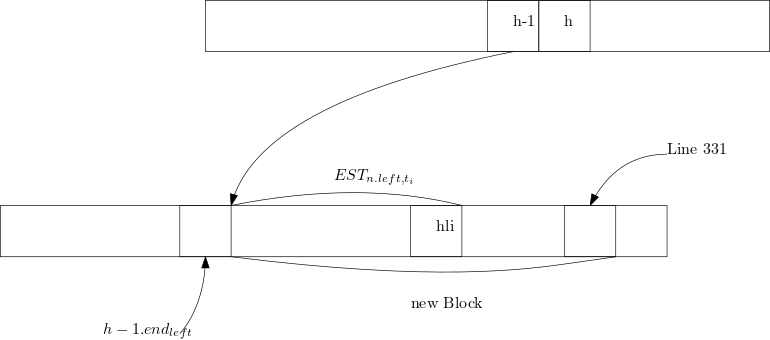
\includegraphics[width=5in]{pics/trueRefresh}
  \caption{New established operations of the left child are in the new block.}
\end{figure}
\begin{lemma}[Precise True Refresh] \label{lem::prectrueRefresh}
  Let $t_i$ be the time an instance of \nf{n.Refresh()} read the head (Line \ref{readHead}) and $t_t$ be the time its \nf{TryAppend(new, s)} terminates with  and returns \nf{true} (Line \ref{cas}). We have \nf{ops(EST\sub{n.left, t\sub{i}})} $\cup$ \nf{ops(EST\sub{n.right, t\sub{i}})} $\subseteq$ \nf{ops(n.blocks)}.
\end{lemma}
%\it{Mention this new block is establish in t\sub{t}. last sentece is not complete}

%\begin{lemma}[falseRefresh] \label{lem:falseRefresh}
%    If instance \nf{r} of \nf{n.Refresh()} reads value \nf{s} on line \ref{readHead} and then returns \nf{false}, then there is another instance $r^\prime$ of \nf{n.Refresh()} that has performed a successful \nf{TryAppend(new, s)}. A \nf{TryAppend()} is successful if its \nf{CAS} is successful.
%\end{lemma}
%\begin{proof}
%  If there is no other concurrent successful \nf{n.Refresh()} then \nf{n.Refresh()} would succeed in Line 313. So there is another \nf{n.Refresh()}, that has appended its block in \nf{n.blocks[h]} after Line 310 of the first \nf{n.Refresh()}. 
%%Otherwise the other \nf{Refresh(n)} should have read \nf{h$^\prime$>h} instead of \nf{h} for \nf{n.head}(Line 52).
%\end{proof}

\pagebreak


\begin{lemma}[Double Refresh] \label{doubleRefresh}
  Consider two consecutive failed instances $R_1$, $R_2$ of \nf{n.Refresh()} by some process. Let $t_1$ be the time $R_1$ is invoked and $t_2$ be the time $R_2$ terminated. We have \nf{ops(EST\sub{n.left, t\sub{1}})} $\cup$ \nf{ops(EST\sub{n.right, t\sub{1}})} $\subseteq$ \nf{ops(EST\sub{n, t\sub{2}})}.
\end{lemma}
\begin{proof}
  

If Line \ref{cas} of $R_1$ or $R_2$ returns \nf{true}, then the claim is held by Lemma~\ref{lem::trueRefresh}. Let $R_1$ read $i$ and $R_2$ read $i+1$ from Line \ref{readHead}. If $R_2$ reads some value greater than $i+1$ in Line \ref{readHead} it means a successful instance of \nf{Refresh()} started after Line \ref{readHead} of $R_1$ and finished its Line \ref{incrementHead1} or \ref{incrementHead2} before \ref{readHead} of $R_2$, from Lemma~\ref{lem::trueRefresh} by the end of this instance \nf{ops(EST\sub{n.left, t\sub{1}})} $\cup$ \nf{ops(EST\sub{n.right, t\sub{1}})} has been propagated.

Since $R_2$'s \nf{TryAppend()} returns \nf{false} then there is another successful instance $R_2^\prime$ of \nf{n.Refresh()} that has done \nf{TryAppend()} successfully into \nf{n.blocks[i+1]} before $R_2$ tries to append. In Figure 1 we see why the block $R_2^\prime$ is appending contains established block in the n's children at $t_1$, since it create a block reading the head after $t_1$. By Lemma \ref{lem::prectrueRefresh} after $R_2^\prime$'s \nf{CAS} we have \nf{ops(EST\sub{n.left, t\sub{1}})} $\cup$ \nf{ops(EST\sub{n.right, t\sub{1}})} $\subseteq$ \nf{ops(n.blocks)}. Also by Lemma \ref{lem::headInc} of $R_2$  head is more than $i+1$ after $R_2$\'s \ref{incrementHead2} line, so the block appended by $R_2^\prime$ to \nf{n} is established by then. To summarized $t_1$ is before $R_2^\prime$'s read head and $R_2^\prime$'s \nf{CAS} is before $R_2$'s termination. So \nf{ops(EST\sub{n.left, t\sub{1}})} $\cup$ \nf{ops(EST\sub{n.right, t\sub{1}})} $\subseteq$ \nf{ops(EST\sub{n, t\sub{2}})}.
%It is obvious that the \nf{new} constructed by the second Refresh in Line 36 contains the blocks in \nf{new} by $R_1$ which $R_1^\prime$ did not contain, since \nf{n.head} is only increasing (Maybe Lemma~\ref{lem::oldnewOrder}). If $R_2$ succeeds by Lemma~\ref{lem::trueRefresh} the claim holds. If not, it is deduced that \nf{n.blocks[h]} was not \nf{null} before $R_2$'s \nf{CAS}. Furthermore, \nf{n.blocks[h]} was \nf{null} before reading \nf{h} by $R_1$. So there is a successful \nf{Refresh()} after the read of \nf{h} in $R_1$ and before the \nf{CAS} of $R_2$. This \nf{Refresh()} contains all the new established operations before Line 35 (Maybe Lemma~\ref{lem::oldnewOrder}) and by Lemma~\ref{lem::trueRefresh} our claim holds. See Figure~\ref{}.
\end{proof}
\it{last sentence need more detail and should be earlier. define i and tell why R2prime exists}

\begin{figure}[hbt]
  \center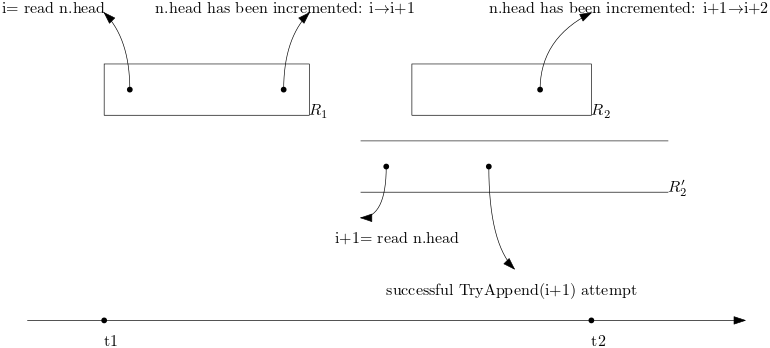
\includegraphics[width=6in]{pics/compactdouble.png}
  \caption{$t1<$ $r_1$ reading head $<$ incrementing \nf{n.head} from $i$ to $i+1$ $<$ $R_2^\prime$ reading head $<$ \nf{TryAppend(i+1)} $<$ incrementing \nf{n.head} from $i+1$ to $i+2$ $<t2$}
\end{figure}
\it{this chain with more depth should be in the proof}

%  Block \nf{new} is created of new established subblocks of children of \nf{n}(Lemma \ref{lem::createBlock}, Line 46). If \nf{CAS} in Line 48 succeeds then by Lemma~\ref{lem::trueRefresh} new established blocks will be in \nf{n}.
  
\pagebreak


\begin{corollary}[Propagate Step] \label{doublyRefresh}
All operations in \nf{n}'s children's established blocks before line \ref{firstRefresh} are guaranteed to be in \nf{n}'s established blocks after line~\ref{secondRefresh}.
\end{corollary}
\begin{proof}
Lines \ref{firstRefresh} and \ref{secondRefresh} satisfy the preconditions of Lemma \ref{doubleRefresh}.
\end{proof}

\begin{corollary}
  After \nf{Append(blk)} finishes \nf{ops(blk)}$\subseteq$\nf{ops(root.blocks[x])} for some \nf{x} and only one \nf{x}.
\end{corollary}
\begin{proof}
  Follows from Lemma \ref{doubleRefresh}, \ref{append}.
\end{proof}

\pagebreak


\begin{lemma}[Block Size Upper Bound]\label{blockSize}
Each block contains at most one operation from each processs.
\end{lemma}
\begin{proof}
By proof of contradiction, assume there are more than one operation from process $p$ in block $b$ in node $n$. A process cannot invoke more than one operations concurrently. From $p$ 's operations in $b$, let $op_1$ be the first operation invoked and $op_2$ be the second one. Note that it is terminated before $op_2$ started. So before appending $op_2$ to the tree $op_1$ exists in every node from the path of $p$'s leaf to the root. So there is some block $b^\prime$  before $b$ in $n$ containing $op_1$. $op_1$ existing in $b$ an $b^\prime$ contradicts with \ref{append}.
\end{proof}

\begin{lemma}[Subblocks Upperbound]\label{subBlocksBound}
Each block has at most $p$ direct subblocks.
\end{lemma}
\begin{proof}
  It follows directly from Lemma \ref{blockSize} and the observation that each block contains at least one operation, induced from Line~\ref{addOP}. 
\end{proof}


\pagebreak


\begin{definition} [Ordering of operations inside the nodes] \label{ordering}
$\blacktriangleright$ Note that processes are numbered from 1 to $p$, left to right in the leaves of the tree and from Lemma \ref{blockSize} we know there is at most one operation from each process in a given block.

\begin{itemize}
\item We call operations strictly before $op$ in the sequence of operations $S$, prefix of the $op$.
  \item $E(n,b)$ is the sequence of enqueue operations $\in$ \nf{ops(n.blocks[b])} ordered by their process id.
  \item $E_{n,b,i}$ is the $i$th enqueue in $E(n,b)$.
  \item $D(n,b)$ is the sequence of dequeue operations $\in$ \nf{ops(n.blocks[b])} ordered by their process id.
  \item $D_{n,b,i}$ is the $i$th enqueue in $D(n,b)$.
\item Order of the enqueue operations in $n$: $E(n)=E(n,1).E(n,2).E(n,3)...$
\item $E_{n,i}$ is the $i$th enqueue in $E(n)$.
\item Order of the dequeue operations in $n$: $D(n)=D(n,1).D(n,2).D(n,3)...$
\item $D_{n,i}$ is the $i$th dequeue in $D(n)$.
\item Linearization: $L=E(root,1).D(root,1).E(root,2).D(root,2).E(root,3).D(root,3)...$
\end{itemize}
\end{definition}
\it{Note that in the non-root nodes we only order enqueues and dequeues among the operations of their own type. Since \nf{GetENQ()} only searches among enqueues and \nf{IndexDEQ()} works on dequeues.}

\pagebreak

\begin{lemma}[Get correctness] \label{get}
If \nf{n.blocks[b].num\sub{enq}$\geq$i} then \nf{n.GetENQ(b,i)} returns $E_{n,b,i}$.
\end{lemma}
\begin{proof}
We are going to prove this lemma by induction on the height of node \nf{n}. The base case, where \nf{n} os a leaf, is straightforward (Line \ref{getBaseCase}). Leaf blocks each contain exactly one operation, so only \nf{n.GetENQ(b,1)} can be called where \nf{n} is a leaf. \nf{n.GetENQ(b,1)} returns the operation stored in the $b$th block of leaf \nf{n}.

For the induction step we prove \nf{n.GetENQ(b,i)} returns $E_{n,b,i}$, if \nf{n.child.GetENQ(b,i)} returns $E_{n.child,b,i}$. For non-leaf nodes it is decided that the \nf{i}th enqueue in block \nf{b} of internal node \nf{n} is in the \nf{n.blocks[b]}'s subblocks in the left child of \nf{n} or in the \nf{n.blocks[b]}'s subblocks in the right child of \nf{n} (line \ref{leftOrRight}). From Definition \ref{ordering} we know enqueue operations in a block are ordered by their process id and since in leaves of the tree are ordered by process id from left to right, thus operations from the left subblocks come before operations from the right subblocks in a block (See Figure \ref{figGet}). Furthermore \nf{b.num\sub{enq-left}} stores the number of \nf{enqueue()} operations from the \nf{n.blocks[b]}'s subblocks in the left child of \nf{n}. So if \nf{i} is greater than \nf{b.num\sub{enq-left}} it means $i$th operation is propagated from the right child, otherwise we should search for the $i$th enqueue in the left child. By definition \ref{def::ops} and \ref{def::subblock} we need to search in subblocks of \nf{n.blocks[b]} from the range \texttt{n.left.blocks[n.blocks[i-1].end\textsubscript{left}+1..n.blocks[i].end\textsubscript{left}]} $\cup$ \texttt{n.right.blocks[n.blocks[i-1].end\textsubscript{right}+1..n.blocks[i].end\textsubscript{right}]}.

If the $i$th \nf{enqueue} of \nf{n.blocks[b]} is in the left child it would be $i$th enqueue in \texttt{n.left.blocks[n.blocks[i-1].end\textsubscript{left}+1..n.blocks[i].end\textsubscript{left}]} by Definition \ref{def::subblock}. Also we know there are $eb=n.blocks[b-1].sum_{enq-left}$ enqueues in the blocks before this range, so $E_{n,b,i}$ is $E_{n.left, i+eb}$, which is $E_{n.left,b^\prime,i^\prime}$ for some $b^\prime$ and $i^\prime$. We can compute $b^\prime$ search for $i+eb$th enqueue in \tt{n.left} and $i^\prime$ is \tt{i+eb-n.left.blocks[}$b^\prime-1$\tt{].sum\sub{enq}}. The parameters in \ref{leftChildGet} are for searching $E_{n.left, i+eb}$ in \nf{n.left.block} in the expected range of blocks, so this \nf{BSearch} returns the index of the subblock containing $E_{n,b,i}$.

Else if the enqueue we are looking for is in the right child then there are \nf{n.blocks[b].num\sub{enq-left}} enqueues ahead of it in \nf{n.blocks[b]} but not in \texttt{n.right.blocks[n.blocks[i-1].end\textsubscript{right}+1..n.blocks[i].end\textsubscript{right}]}. So we need to search for \nf{i-n.blocks[b].num\sub{enq-left}+ n.blocks[b-1].sum\sub{enq-right}} (Line \ref{rightChildGet}). Other parameters are assigned similar for the left child. So in both cases the direct subblock containing $E_{n,b,i}$ is computed in Lines \ref{leftChildGet} and \ref{rightChildGet}.

 Finally, \nf{n.child.GetENQ()} is invoked on the subblock containing $E_{n,b,i}$ which returns $E_{n,b,i}$ by the hypothesis of the induction.
\end{proof}

\begin{figure}[hbt]  
  \center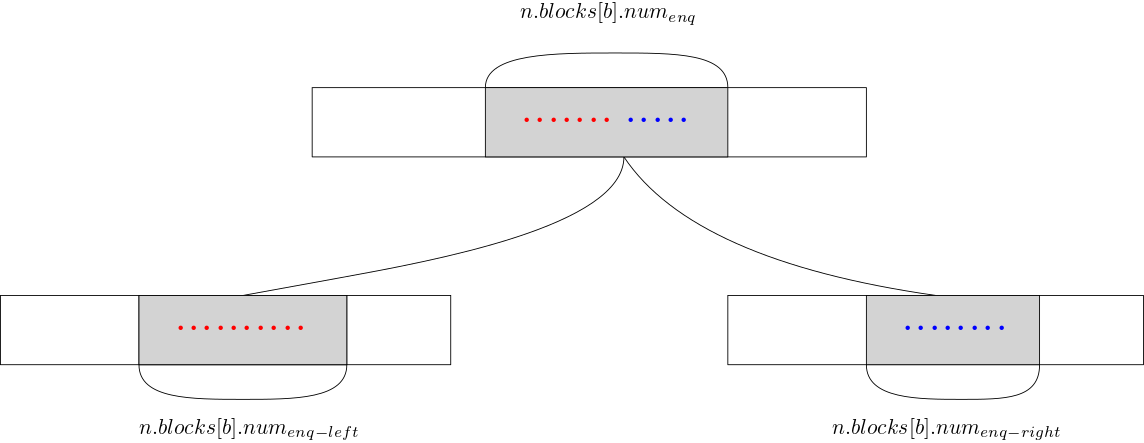
\includegraphics[width=6in]{pics/blockSumEnq.png}
  
  \caption{The number and ordering of the enqueues propagated from the left and the right child to \nf{n.blocks[b]}. Enqueue operations from the left subblocks, colored red, are ordered before the enequeue operations from the right child, colored blue.
  }\label{figGet}
\end{figure}

%\textit{I'm not sure it is going to be long and boring to talk about the parameters, since the reader can find out them.}

\pagebreak


\begin{lemma}[DSearch correctness] \label{dsearch}
Assume \nf{root.blocks[end].sum\sub{enq}}$\geq$\nf{e} and $E_{root, e}$'s \nf{element} is the response to some \nf{Dequeue()} operation in \nf{root.blocks[end]}.  \nf{DSearch(e, end)} returns \nf{<b, i>} such that $E_{root,b,i}= E_{root,e}$.
\end{lemma}
\begin{proof}
It is trivial to see that the doubling search from \nf{root.blocks[end]} to \nf{root.blocks[0]} will find $E_{root,e}$ eventually. Because \nf{root.blocks[].sum\sub{enq}} is an increasing value from 0 to some value greater than \nf{e}. So there is a \nf{b} that \nf{root.blocks[b].sum\sub{enq}}$>e$ but \nf{root.blocks[b-1].sum\sub{enq}}$<e$. 

First we show \nf{end-b}$\leq 2 \times$\nf{root.blocks[b].\size+root.blocks[end].\size+1}. From line \ref{addOP}, we know that size of the every block in the tree is greater than 0. So each block in \nf{root.blocks[b..end]} contains at least one \nf{Enqueue} or at least one \nf{Dequeue}. Suppose there were more than \nf{root.blocks[b].\size}\nf{Dequeue}s in \nf{root.blocks[b+1..end-1]}. Then the  queue would become empty at some point after \nf{blocks[b]}'s last operations and before \nf{root.blocks[end]}'s first operation. Which means the response to to a \nf{Dequeue} in \nf{root.blocks[end]} could not be in $E(n,b)$. Furthermore since the size of the queue would become \nf{root.blocks[end].\size} after the \nf{root.blocks[end]}, there cannot be more than \nf{root.blocks[b].\size + root.blocks[end].\size} \nf{Enqueue}s. Because there can be at most \nf{root.blocks[b].\size}\nf{Dequeue}s and the final size is \nf{root.blocks[end].\size}. Overall there can be at most $2 \times$\nf{root.blocks[b].\size+ root.blocks[end].\size} operations in \nf{root.blocks[b+1..end-1]} and since each block size is $\geq 1$ thus there are at most $2 \times$\nf{root.blocks[b].\size+ root.blocks[end].\size} blocks in between \nf{root.blocks[b]} and \nf{root.blocks[end]}. So \nf{end-b}$\leq 2 \times$\nf{root.blocks[b].\size+root.blocks[end].\size+1}. See Figure \ref{end-b}.

Now that we know there are at most \nf{root.blocks[b].\size+root.blocks[end].\size} blocks in between \nf{root.blocks[b]} and \nf{root.blocks[end]} then with doubling search in $\Theta \big(\log($\nf{root.blocks[b].\size+root.blocks[end].\size}$)\big)$ steps we reach \nf{start=c} that the \nf{root.blocks[c].sum\sub{enq}} is less than \nf{e} and \nf{end-c} is not more than $2\times$\nf{root.blocks[b].\size+root.blocks[end].\size}. Beause otherwise, then \nf{(end-c)/2} satisfied the \nf{root.blocks[(end-c)/2].sum\sub{enq}<e}. In line \ref{doubling} the differnece between \nf{end} and \nf{start} is doubled. See Figure \ref{fig::doubling}.

 After computing \nf{b}, the value \nf{i} is computed via the definition of \nf{sum\sub{enq}} in constant time (Line \ref{DSearchComputei}). So the routine non constant part is the binary search which takes $\Theta(\log$\nf{root.blocks[b].\size+root.blocks[end].\size)}$)$ steps from the first paragraph.

\end{proof}
\begin{figure}[hbt]  
  \center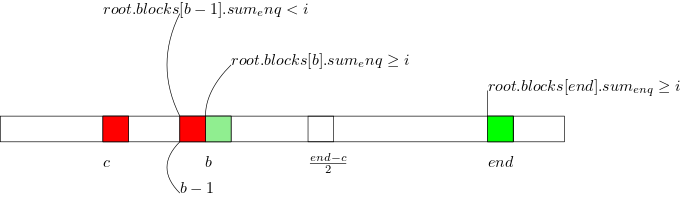
\includegraphics[width=6in]{pics/doubling.png}
  
  \caption{Distance relations between $b,c,end$}
  \label{fig::doubling}
\end{figure}

\begin{figure}[hbt]  
  \center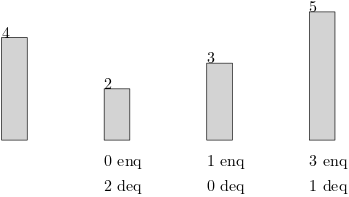
\includegraphics[width=3in]{pics/end-b.png}

  \caption{The number written on top of the bars is the queue size. the first block is $b$ and the last block is $end$.}
  \label{end-b}
\end{figure}

\pagebreak

\begin{lemma}[Index correctness]
 \nf{n.IndexDEQ(b,i)} returns the rank in $D(root)$ of $D_{n,b,i}$.
\end{lemma}
\begin{proof}
We will prove this by induction on the distance of \nf{n} from the \nf{root}. We can see the base case \nf{root.IndexDEQ(b,i)} is trivial (Line \ref{indexBaseCase}).
  In the non-root nodes \nf{n.IndexDEQ(b,i)} computes the superblock of the $i$th Dequeue in the $b$th block of \nf{n} in \nf{n.parent} by Lemma \ref{superBlock} (Line \ref{computeSuper}). After that the order in $D(n.parent, superblock)$ is computed and \nf{index()} is called on \nf{n.parent} recursively. Then if the operation was propagated from the right child the number of dequeues from the left child are added to it (Line \ref{considerRight}), because the left child operations come before the right child operations (Definition \ref{ordering}).
\end{proof}
\textit{Do I need to talk about the computation of the order in the parent which is based on the definition of ordering of dequeues in a block? Make sure to show preconditions of all invocation of \nf{BSearch} are satisfied.}

%\begin{definition}
%An enqueue operation is \textit{finished} if its argument is returned by some process. A dequeue operation is \texttt{finished} if it returns \nf{null} or some value. Block \nf{b} is \textit{done} if all operations in \nf{ops(b)} are finished.
%\end{definition}
%\textit{Problem: we increment the \nf{num\sub{finished}} before returning and after the computing response. How to articulate the sentence above in a not confusing correct way?}
%
%\begin{lemma}[help]\label{help}
%After that \nf{TryAppend()} who is helping finishes, prefix for the blocks of \nf{root.blocks[root.FindMostRecentDone]} are done.
%\end{lemma}

\begin{lemma}[Computing SuperBlock]\label{superBlock}
After computing line \ref{computeSuper} of \nf{n.IndexDEQ(b,i)}, \nf{n.parent.blocks[superblock]} contains $D(n,b,i)$.
\end{lemma}
\begin{proof}
Lemmas 28,29,30,31.
\end{proof}
\begin{lemma}
Value read for \nf{super[b.group]} in line 418 is not null.\end{lemma}
\begin{proof}
  Values \nf{np\textsubscript{dir}} read in lines \ref{setNP}, \nf{super} are set before incrementing in lines \ref{setSuper},\ref{incNP}. So before incrementing \nf{num\sub{propagated}, super[num\sub{propagated}]} is set so it cannot be null while reading.
\end{proof}
\begin{lemma} \nf{super[]} preserves order from child to parent; i.e. if in node \nf{n} block \nf{b} is before \nf{c} then \nf{b.group} $\leq$ \nf{c.group}
\end{lemma}
\begin{proof} Line \ref{setGroup}. Since  \nf{num\sub{propagated}} is increasing.\end{proof}

\begin{lemma} Let \nf{b, c} be in node \nf{n}, if \nf{b.group} $\leq$ \nf{c.group} then \nf{super[b.group]} $\leq$ \nf{super[c.group]}\end{lemma}
\begin{proof} Line \ref{setSuper}.\end{proof}

\begin{lemma}
The number of the \nf{block}s with \nf{group=i} in a node is $\leq p$.  
\end{lemma}
\begin{proof}For the sake of simplicity we assumed all the blocks are propagated from the left child.
\begin{figure}[hbt]
  \center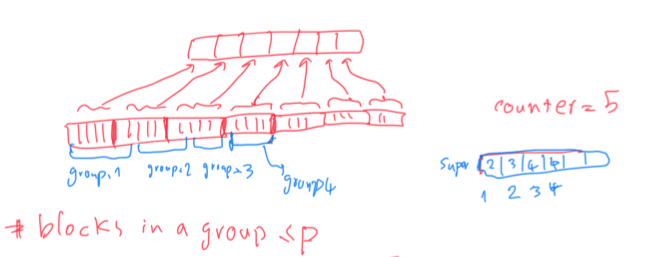
\includegraphics[width=5in]{pics/index1}
\end{figure}  
\end{proof}


% \item In a propagate step at most 2 different time values are read \\ If there are more than 2 numbers then the smallest number should have been propagated far before.
% \item There are at most $p^2$ blocks with same time value in a node. \\ At most p processes could die before line 27 and each contains at most p elements.
\begin{lemma} \nf{super[i+1]-super[i]}$\leq p$\end{lemma}
\begin{proof}
 In a Refresh with successful CAS in line 46, \nf{super} and \nf{counter} are set for each child in lines 48,49. Assume the current value of the counter in node \nf{n} is \nf{i+1} and still \nf{super[i+1]} is not set. If an instance of successful \nf{Refresh(n)} finishes \nf{super[i+1]} is set a new value and a block is added after \nf{n.parent[sup[i]]}. There could be at most $p$ successful unfinished concurrent instances of \nf{Refresh()} that have not reached line 49. So the distance between \nf{super[i+1]} and \nf{super[i]} is less than $p$.
 \begin{figure}[hbt]
  \center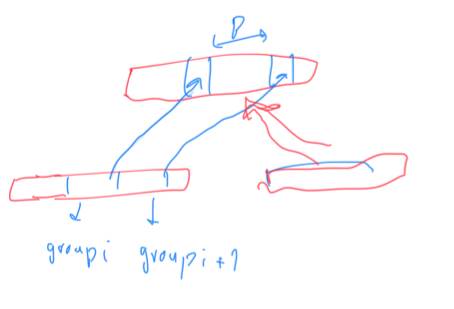
\includegraphics[width=4in]{pics/index2}
\end{figure}  
\end{proof}
\begin{lemma}[super property]\label{superCounter}
If \nf{super[i] $\neq$ null} in node \nf{n}, then \nf{super[i]} is the index of the superblock of a block with \nf{time=i} in \nf{n.parent.blocks}.
\end{lemma}
\begin{lemma}\label{superRange} Superblock of \nf{b} is within range $\pm 2p$ of the \nf{super[b.time]}.
\end{lemma}

\begin{proof} \nf{super[i]} is the index of the superblock of a block containing block b, followed by Lemma \ref{superCounter}. \nf{super(b)} is the real superblock of b. \nf{super(t]} is the index of the superblock of the last block with time \nf{t}. If \nf{b.time} is \nf{t} we have:
$$super[t]-p\leq super[t-1]\leq super(t-1] \leq super(b) \leq super(t+1)\leq super(t+1]\leq super[t]+p$$
\end{proof}

\begin{lemma}
Search in each level of \nf{IndexDeq()} takes $O(\log p)$ steps.  
\end{lemma}
\begin{proof}
Show preconditions are satisfied and the range is $p$.  
\end{proof}

\pagebreak



%\begin{lemma}[Search Ranges]\label{search}
%  Preconditions of all invocation of \nf{BSearch} are satisfied.
%\end{lemma}
%\begin{proof}
%  
%Line 83: \nf{Get(i)} is called if the result of a dequeue is not null. The search is among all blocks in the root.
%
%Line 88: This search tries to find the ith enqueue, knowing that it is in the left child. Search is done over the left subblocks. The start and end of the range are followed by definition. Line 92 is the same.
%
%Line 101: Here, the goal is to find the superblock. We know the distance between answer and the \nf{super[i]} is at most $p$, since at most $p$ processes could die.
%
%\end{proof}

\begin{definition}
In an execution on a queue, the dequeue operations that return some value are called \it{non-null dequeues}.  
\end{definition}
\begin{observation} \label{responseToADeq}
$k$th non-null dequeue in an execution returns the \nf{element} of $k$th enqueue.
\end{observation}

\begin{lemma}\label{sizeCorrectness}
  \nf{root.blocks[b].\size}is the \size of the queue if the operations in the prefix for the $b$th block in the root are applied with the order of $L$.  
\end{lemma}
\begin{proof}
If the \size of a queue is greater than 0 then a \nf{Dequeue()} would decrease the \size of the queue, otherwise the \size of the queue remains 0. By definition  of $L$ in definition \ref{ordering} enqueue operations come before dequeue operations in a block. If the queue won't become empty after $b$th block we can compute the size of the queue after $b$th block using with this equality \nf{root.blocks[b].size= root.blocks[b-1].size+ root.blocks[b].sum\sub{enq}- root.blocks[b].sum\sub{deq}} (Line \ref{computeLength}). Otherwise \nf{root.blocks[b-1].size+ root.blocks[b].sum\sub{enq}- root.blocks[b].sum\sub{deq}} would become negative. Since there are more dequeue operations than the size of the queue. See table \ref{qhistory}.
\end{proof}

\begin{lemma} \label{numberOfNND}
If the operations are applied with the order of $L$, the number of non-null dequeues in the prefix for a block \nf{b} is \nf{b.sum\sub{enq}-b.\size}
\end{lemma}
\begin{proof}
If there are $enqs$ enqueue operations in the prefix for \nf{b}, then the size of the queue after  prefix for \nf{b} is \nf{enqs - non-null deqs} by Observation 35. The correctness of the feild \size is showed in Lemma \ref{sizeCorrectness}.
\end{proof}

\begin{lemma}\label{nullReturn}
$D_{root,b,i}$ returns \nf{null} iff \nf{root.blocks[b-1].\size+ root.blocks[b].num\sub{enq}- i <0}.
\end{lemma}


\begin{lemma}[Computing Response] \label{computeHead}
  Let $S$ be the state of an empty queue if the operations in $L$ are applied on it. \nf{FindResponse(b,i)} returns the element that is the the response to $D_{root,b,i}$ in $S$. If the queue is empty in $S$ then it returns \nf{null}.
\end{lemma}
\begin{proof}
First note that by Definition \ref{ordering} the linearization ordering  of operations will not change as new operations come so instead of talking about the linearization of operations before the $E_{root, b, i}$ we talk about what if the whole operation in the linearization are applied on a queue.

$D_{root,b,i}$ is $D_{root,root.blocks[b-1].sum_{deq}+i}$ from the definition \ref{ordering} and \it{$sum_{enq}$}.  $D_{root,b,i}$ returns \nf{null} if \nf{root.blocks[b-1].\size+ root.blocks[b].num\sub{enq}- i <0} by Lemma \ref{nullReturn} (Line \ref{checkEmpty}). Otherwise if it is $d^\prime$th non-null dequeue in $L$ it returns $d^\prime$th enqueue by Observation \ref{responseToADeq} . By Lemma \ref{numberOfNND} there are \nf{root.blocks[b-1].sum\sub{enq} - root.blocks[b-1].\size} non-null dequeue operations before prefix for \nf{root.blocks[b-1]}. Note that the dequeues in \nf{root.blocks[b]} before the $i$th dequeue are non-null dequeues. So the response is $E_{root,i - root.blocks[b-1].size + root.blocks[b-1].sum\sub{deq}}$ (Line \ref{computeE}). See figure \ref{computeResponseDetail}.

After computing \nf{e} we can find \nf{b,i} such that $E_{root,b,i}=E_{root,e}$ using \nf{DSearch} and then find its \nf{element} using \nf{GetEnq} (Line \ref{findAnswer}).
\end{proof}

\begin{figure}[hbt]  
  \center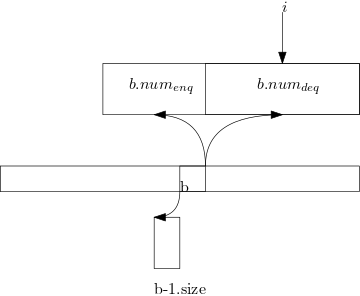
\includegraphics[width=2in]{pics/computeResponseDetail.png}\caption{The position of $E_{root,b,i}$.}
\label{computeResponseDetail}
\end{figure}

\begin{table}[hbt]
\centering
  \begin{tabular}{c|c|c|c|c}
    \hline &\texttt{DEQ()} & \texttt{ENQ(5)}, \texttt{ENQ(2)}, \texttt{ENQ(1)}, \texttt{DEQ()}& \texttt{ENQ(3)}, \texttt{DEQ()}&  \texttt{ENQ(4)}, \texttt{DEQ()}, \texttt{DEQ()}, \texttt{DEQ()}, \texttt{DEQ()}\\ \hline
    \#enqueues & 0 & 3 & 1 & 1 \\ \hline
        \#dequeues & 1 & 1 & 1 & 4 \\ \hline
            \#non-null dequeues & 0 & 1 & 2 & 5 \\ \hline
                size & 0 & 2 & 2 & 0 \\ \hline
  \end{tabular}
  \caption{An example of root blocks fields. Blocks are from left to right and operations in the blocks are also from the left to right.}\label{qhistory}
\end{table}


%\begin{proof}
%  \nf{head} is incremented in lines 51, 54 after trying to append a block to the index of the last \nf{head} read. If it was successful, we have to do this, but if it was unsuccessful, it means it has appended to the index before, so we have to update the \nf{head}. If a process dies before line 51, another process will increment \nf{head} in line 54.
%\end{proof} 

\pagebreak

\begin{theorem}[Main]
The queue implementation is linearizable.
\end{theorem}
\begin{proof}
  We choose $L$ in Definition \ref{ordering} to be linearization ordering of operations and prove if we linearize operations as $L$ the queue works consistently.
\end{proof}
%\begin{lemma}
%Operations in a block have a time point in common (There is a time $t$ all the operations are running).
%\end{lemma}

\begin{lemma}[satisfiability]
$L$ can be a linearization ordering.
\end{lemma}
\begin{proof}
To show this we need to say if in an execution, \nf{op\sub{1}} terminates before \nf{op\sub{2}} starts then \nf{op\sub{1}} is linearized before \nf{op\sub{2}}. If \nf{op\sub{1}} terminates before \nf{op\sub{2}} starts it means \nf{op\sub{1}.Append()} is terminated before \nf{op\sub{2}.Append()} starts. From Lemma \ref{append} \nf{op\sub{1}} is in \nf{root.blocks} before \nf{op\sub{2}} propagates so \nf{op\sub{1}} is linearized before \nf{op\sub{2}} by Definition \ref{ordering}.

Once some operations are aggregated in one block they will be propagated together up to the root and we can linearize them in any order among themselves. Furthermore in L we arbitrary choose the order to be by process id, since it makes computations in the blocks faster .
\end{proof}

\begin{lemma}[correctness]
  If operations are applied as $L$ on a sequential queue, the sequence of the responses would be the same as our algorithm.
\end{lemma}

\begin{proof}
\it{Old parts to review}
  We show that the ordering $L$ stored in the root, satisfies the properties of a linearizable ordering.
  \begin{enumerate}
    \item If $op_1$ ends before $op_2$ begins in $E$, then $op_1$ comes before $op_2$ in $T$.\\$\blacktriangleright$ This is followed by Lemma \ref{append}. The time $op_1$ ends it is in root, before $op_2$, by Definition \ref{ordering} $op_1$ is before $op_2$.
    \item Responses to operations in $E$ are same as they would be if done sequentially in order of $L$. \\$\blacktriangleright$ Enqueue operations do not have any response so it does no matter how they are ordered. It remains to prove  Dequeue $d$ returns the correct response according to the linearization order. By Lemma \ref{computeHead} it is deduced that the head of the queue at time of the linearization of $d$ is computed properly. If the Queue is not empty by Lemma \ref{get} we know that the returning response is the computed index element.
  \end{enumerate} 
\end{proof}

\pagebreak


\begin{lemma}[Amortized time analysis]
%  \nf{n.GetEnq(b,i), n.Index(b,i)} take $O(\log^2 p)$ steps. Search in the root may take $O(\log Q+ p^2)$ steps. Helping is done every $p^2$ block appended to the root and takes $p\times \log^2p$ steps. Amortized time consumed for helping by each process is $O(\log^2 p)$.
\nf{Enqueue()} and \nf{Dequeue} take $O(\log^2 p +q)$ steps (amortized anlysis), which $p$ is the number of processes and $q$ is the size of the queue at the time of invocation.
\end{lemma}
\begin{proof}
\nf{Enqueue(x)} consists of creating a \nf{block(x)} and appending it to the tree. The first part takes constant time. To propagate \nf{x} to the root the algorithm tries two \nf{Refresh}es in each node of the path from the leaf to the root (Lines \ref{firstRefresh}, \ref{secondRefresh}). Each \nf{Refresh} takes $O(1)$ steps since creating a block is done in constant time and does $O(1)$ \nf{CAS}es. Since the height of the tree is $O(\log p)$, \nf{Enqueue(x)} takes $O(\log p)$ steps.

A \nf{Dequeue()} creates a block with null value element, appends it to the tree, computes its order among operations, and returns the response. The first two part is similar to an \nf{Enqueue} operation. To compute the order there are some constant steps and \nf{IndexDeq} is called. \nf{IndexDeq} does a search with range $p$ in each level (Lemma \ref{superRange}) which takes $O(log^2 p)$ in the tree. In the \nf{FindResponse()} routine \nf{DSearch()} in the root takes $\Theta(\log$(\nf{root.blocks[b].\size+root.blocks[end].\size}) by Lemma \ref{dsearch}, which is $O(\log$ size of the queue when \nf{enqueue} is invoked$)+\log$ size of the queue when \nf{dequeue} is invoked$)$. Each search in \nf{GetEnq()} takes $O(\log p)$ since there are $\leq p$ subblocks in a block (Lemma \ref{subBlocksBound}), so \nf{GetEnq()} takes $O(\log^2 p)$ steps.

If we split \nf{DSearch} time cost between the corresponding \nf{Enqueue}, \nf{Dequeue}, in amortized we have \nf{Enqueue} takes $O(\log p +q)$ and \nf{Dequeue} takes $O(\log^2 p +q)$ steps.
\end{proof}


%\begin{lemma}[Root search range]\label{rootRange}
%  \nf{root.size-root.FindMostRecentDone()} is $O(p^2+q)$, which $p$ is \# processes and $q$ is the \size of the queue.
%\end{lemma}
\end{document}






